\section{Proposed Approach}
\label{sec:approach}
The input  (Figure \ref{fig_sysarch}) is a feature-based CAD model represented by  ($\cup_qf^3$), where `$\cup$' denotes a collection, of `$q$' features (`$f$') having dimensionality `$3$' (solids). In practice, the thin-walled CAD models come in various types, such as mesh, solid, feature-based CAD, etc. This research, as it leverages feature information \cite{YogeshCOEP2013}, expects a feature-based CAD model as input. This, at times can be deemed as limitation, in case of unavailability due to format restrictions, proprietary data etc. But, techniques such as segmentation, feature recognition (FR), can be used effectively to convert the non-feature-based model to a feature-based one.

%\smallskip

\begin{minipage}[c]{\linewidth}
    \begin{minipage}[c]{0.45\linewidth}
\begin{itemize}[noitemsep,topsep=2pt,parsep=2pt,partopsep=2pt,leftmargin=*]
%\item \textbf{Input}: Feature-based CAD models, which are widely available in most of the commercial CAD applications. It is represented by  ($\cup_qf^3$), where `$\cup$' denotes a collection, of `$q$' features (`$f$') having dimensionality `$3$' (solids). Thin-walled CAD models come in various representations, such as mesh, solid, feature-based, etc. This research expects a feature-based CAD model, which can be deemed as limitation in case of its unavailability. But, techniques, such as segmentation, decomposition, feature recognition (FR), etc. can convert a non-feature-based representation to the feature-based CAD model.

\item \textbf{Defeaturing ($\cup_rf^3, r \leq q$) }:  Computes gross shape by removing irrelevant/superficial features \cite{YogeshIITM2013}, using Feature taxonomy and size-based Remnant feature approach (\cite{YogeshCADConf2015}). 

\item \textbf{Generalization ($\cup_rL^3$) }: ``ABEL'' transforms form-features to ``Loft/Sweep'' representations ($L$), making it simpler to develop a generic, portable algorithm (\cite{YogeshIITG2014}). 

\item \textbf{Decomposition}: Cellular decomposition is performed at each feature step to form a graph of nodes having non-volumetrically-overlapping cellular bodies with respective owner-Sweep feature. 

\item \textbf{Midsurface Computation}: Using topology of the graph, the nodes are classified into midsurface-patch generating nodes (solid cells - $sCell$s) and interaction-resolving nodes (interface cells - $iCell$s). Midsurface patch is computed by, first, extracting the profile and the guide curve from the owner Sweep feature, then either offsetting the profile in case of shorter guide curve or sweeping the midcurve \cite{YogeshETES2014,YogeshIJCAET2017} along the guide curve.

\item \textbf{Validation}:  Midsurface needs to  mimic the input shape, faithfully. A novel topological method is used to validate correctness of the midsurface (\cite{YogeshCADandA2015}).

%\item \textbf{Output}: A well-connected midsurface is then sent to downstream applications such as CAE analysis.
\end{itemize}



    \end{minipage}
    \hfill
    \begin{minipage}[c]{0.5\linewidth}
	\centering 
	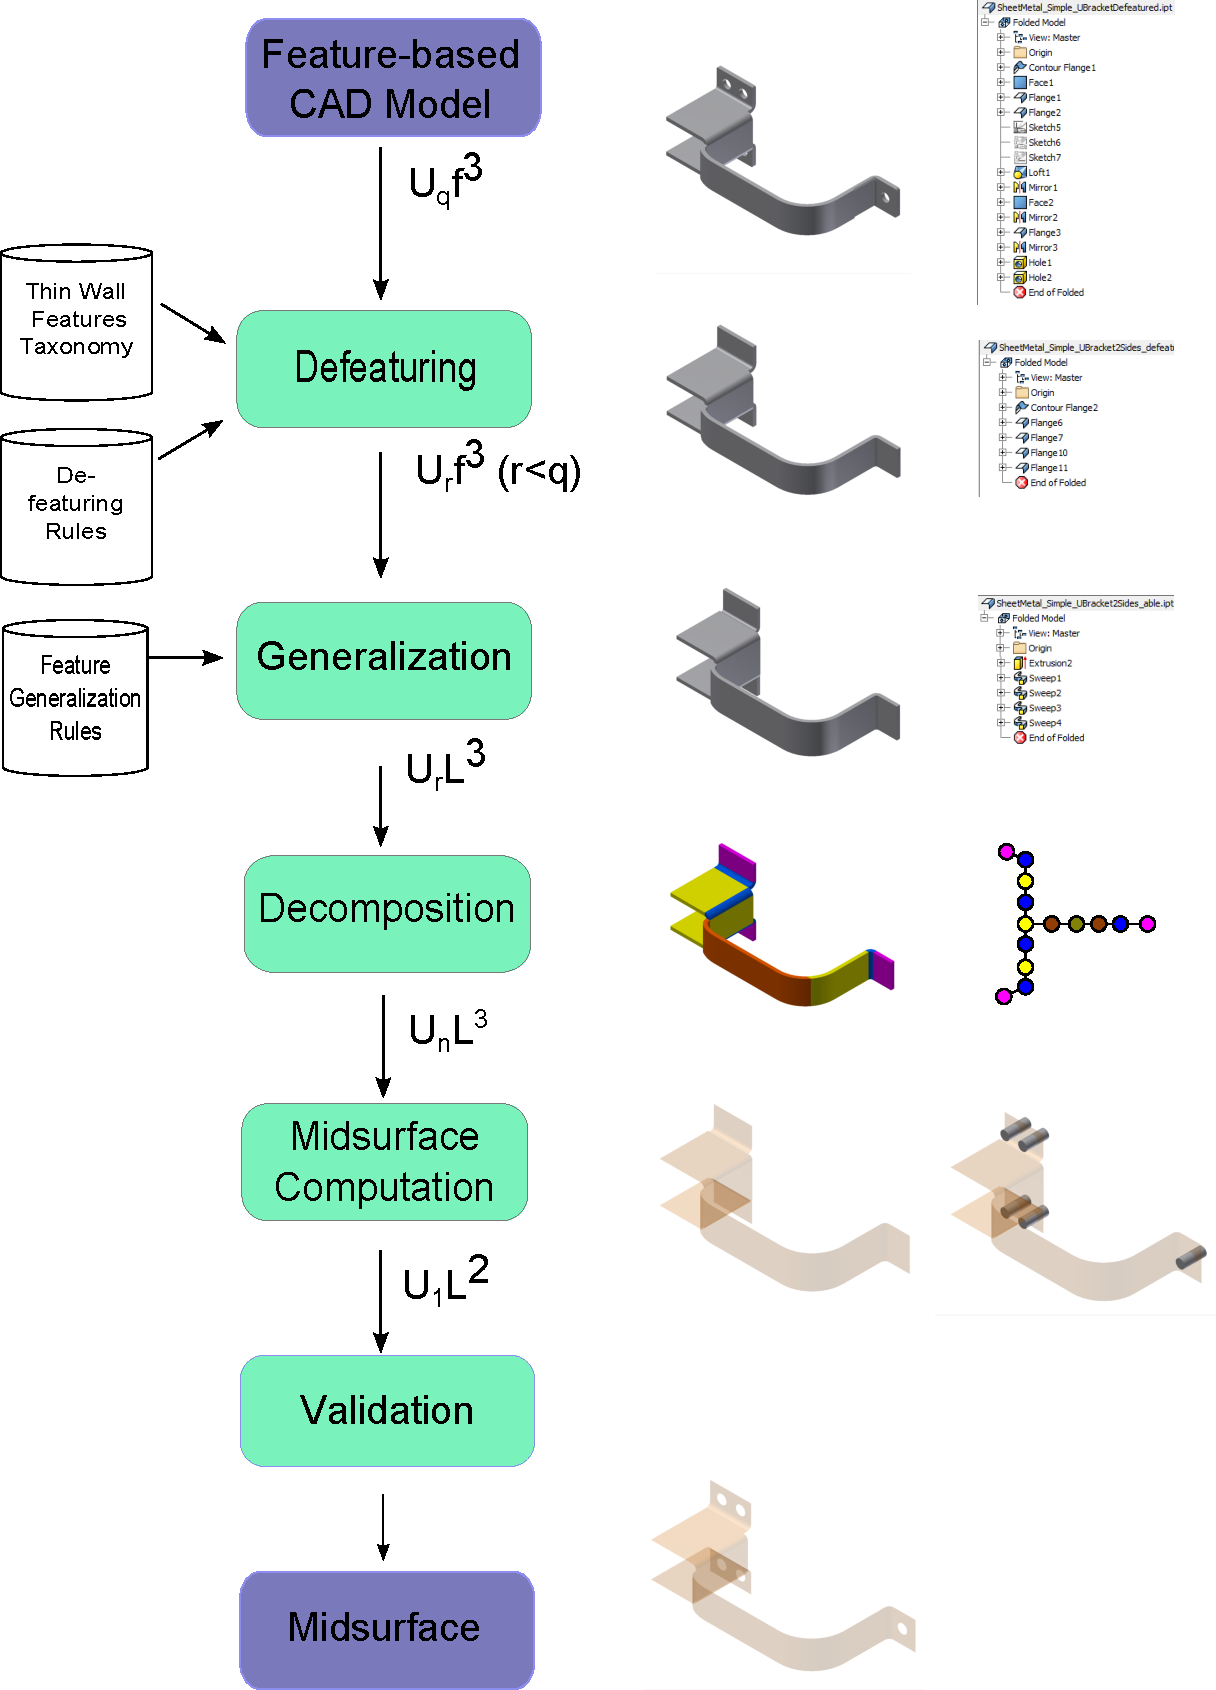
\includegraphics[width=0.95\linewidth]{images/SystemArchitecture3.pdf}
	\captionof{figure}{Overall work-flow}
	\label{fig_sysarch}
    \end{minipage}

\end{minipage}    

A well-connected output midsurface is then sent to downstream applications such as CAE analysis. 

%\bigskip


